
%% bare_conf.tex
%% V1.3
%% 2007/01/11
%% by Michael Shell
%% See:
%% http://www.michaelshell.org/
%% for current contact information.
%%
%% This is a skeleton file demonstrating the use of IEEEtran.cls
%% (requires IEEEtran.cls version 1.7 or later) with an IEEE conference paper.
%%
%% Support sites:
%% http://www.michaelshell.org/tex/ieeetran/
%% http://www.ctan.org/tex-archive/macros/latex/contrib/IEEEtran/
%% and
%% http://www.ieee.org/

%%*************************************************************************
%% Legal Notice:
%% This code is offered as-is without any warranty either expressed or
%% implied; without even the implied warranty of MERCHANTABILITY or
%% FITNESS FOR A PARTICULAR PURPOSE! 
%% User assumes all risk.
%% In no event shall IEEE or any contributor to this code be liable for
%% any damages or losses, including, but not limited to, incidental,
%% consequential, or any other damages, resulting from the use or misuse
%% of any information contained here.
%%
%% All comments are the opinions of their respective authors and are not
%% necessarily endorsed by the IEEE.
%%
%% This work is distributed under the LaTeX Project Public License (LPPL)
%% ( http://www.latex-project.org/ ) version 1.3, and may be freely used,
%% distributed and modified. A copy of the LPPL, version 1.3, is included
%% in the base LaTeX documentation of all distributions of LaTeX released
%% 2003/12/01 or later.
%% Retain all contribution notices and credits.
%% ** Modified files should be clearly indicated as such, including  **
%% ** renaming them and changing author support contact information. **
%%
%% File list of work: IEEEtran.cls, IEEEtran_HOWTO.pdf, bare_adv.tex,
%%                    bare_conf.tex, bare_jrnl.tex, bare_jrnl_compsoc.tex
%%*************************************************************************

% *** Authors should verify (and, if needed, correct) their LaTeX system  ***
% *** with the testflow diagnostic prior to trusting their LaTeX platform ***
% *** with production work. IEEE's font choices can trigger bugs that do  ***
% *** not appear when using other class files.                            ***
% The testflow support page is at:
% http://www.michaelshell.org/tex/testflow/



% Note that the a4paper option is mainly intended so that authors in
% countries using A4 can easily print to A4 and see how their papers will
% look in print - the typesetting of the document will not typically be
% affected with changes in paper size (but the bottom and side margins will).
% Use the testflow package mentioned above to verify correct handling of
% both paper sizes by the user's LaTeX system.
%
% Also note that the "draftcls" or "draftclsnofoot", not "draft", option
% should be used if it is desired that the figures are to be displayed in
% draft mode.
%
\documentclass[conference]{IEEEtran}
\usepackage{blindtext, graphicx}
% Add the compsoc option for Computer Society conferences.
%
% If IEEEtran.cls has not been installed into the LaTeX system files,
% manually specify the path to it like:
% \documentclass[conference]{../sty/IEEEtran}





% Some very useful LaTeX packages include:
% (uncomment the ones you want to load)


% *** MISC UTILITY PACKAGES ***
%
%\usepackage{ifpdf}
% Heiko Oberdiek's ifpdf.sty is very useful if you need conditional
% compilation based on whether the output is pdf or dvi.
% usage:
% \ifpdf
%   % pdf code
% \else
%   % dvi code
% \fi
% The latest version of ifpdf.sty can be obtained from:
% http://www.ctan.org/tex-archive/macros/latex/contrib/oberdiek/
% Also, note that IEEEtran.cls V1.7 and later provides a builtin
% \ifCLASSINFOpdf conditional that works the same way.
% When switching from latex to pdflatex and vice-versa, the compiler may
% have to be run twice to clear warning/error messages.






% *** CITATION PACKAGES ***
%
%\usepackage{cite}
% cite.sty was written by Donald Arseneau
% V1.6 and later of IEEEtran pre-defines the format of the cite.sty package
% \cite{} output to follow that of IEEE. Loading the cite package will
% result in citation numbers being automatically sorted and properly
% "compressed/ranged". e.g., [1], [9], [2], [7], [5], [6] without using
% cite.sty will become [1], [2], [5]--[7], [9] using cite.sty. cite.sty's
% \cite will automatically add leading space, if needed. Use cite.sty's
% noadjust option (cite.sty V3.8 and later) if you want to turn this off.
% cite.sty is already installed on most LaTeX systems. Be sure and use
% version 4.0 (2003-05-27) and later if using hyperref.sty. cite.sty does
% not currently provide for hyperlinked citations.
% The latest version can be obtained at:
% http://www.ctan.org/tex-archive/macros/latex/contrib/cite/
% The documentation is contained in the cite.sty file itself.






% *** GRAPHICS RELATED PACKAGES ***
%
\ifCLASSINFOpdf
  % \usepackage[pdftex]{graphicx}
  % declare the path(s) where your graphic files are
  % \graphicspath{{../pdf/}{../jpeg/}}
  % and their extensions so you won't have to specify these with
  % every instance of \includegraphics
  % \DeclareGraphicsExtensions{.pdf,.jpeg,.png}
\else
  % or other class option (dvipsone, dvipdf, if not using dvips). graphicx
  % will default to the driver specified in the system graphics.cfg if no
  % driver is specified.
  % \usepackage[dvips]{graphicx}
  % declare the path(s) where your graphic files are
  % \graphicspath{{../eps/}}
  % and their extensions so you won't have to specify these with
  % every instance of \includegraphics
  % \DeclareGraphicsExtensions{.eps}
\fi
% graphicx was written by David Carlisle and Sebastian Rahtz. It is
% required if you want graphics, photos, etc. graphicx.sty is already
% installed on most LaTeX systems. The latest version and documentation can
% be obtained at: 
% http://www.ctan.org/tex-archive/macros/latex/required/graphics/
% Another good source of documentation is "Using Imported Graphics in
% LaTeX2e" by Keith Reckdahl which can be found as epslatex.ps or
% epslatex.pdf at: http://www.ctan.org/tex-archive/info/
%
% latex, and pdflatex in dvi mode, support graphics in encapsulated
% postscript (.eps) format. pdflatex in pdf mode supports graphics
% in .pdf, .jpeg, .png and .mps (metapost) formats. Users should ensure
% that all non-photo figures use a vector format (.eps, .pdf, .mps) and
% not a bitmapped formats (.jpeg, .png). IEEE frowns on bitmapped formats
% which can result in "jaggedy"/blurry rendering of lines and letters as
% well as large increases in file sizes.
%
% You can find documentation about the pdfTeX application at:
% http://www.tug.org/applications/pdftex





% *** MATH PACKAGES ***
%
%\usepackage[cmex10]{amsmath}
% A popular package from the American Mathematical Society that provides
% many useful and powerful commands for dealing with mathematics. If using
% it, be sure to load this package with the cmex10 option to ensure that
% only type 1 fonts will utilized at all point sizes. Without this option,
% it is possible that some math symbols, particularly those within
% footnotes, will be rendered in bitmap form which will result in a
% document that can not be IEEE Xplore compliant!
%
% Also, note that the amsmath package sets \interdisplaylinepenalty to 10000
% thus preventing page breaks from occurring within multiline equations. Use:
%\interdisplaylinepenalty=2500
% after loading amsmath to restore such page breaks as IEEEtran.cls normally
% does. amsmath.sty is already installed on most LaTeX systems. The latest
% version and documentation can be obtained at:
% http://www.ctan.org/tex-archive/macros/latex/required/amslatex/math/





% *** SPECIALIZED LIST PACKAGES ***
%
%\usepackage{algorithmic}
% algorithmic.sty was written by Peter Williams and Rogerio Brito.
% This package provides an algorithmic environment fo describing algorithms.
% You can use the algorithmic environment in-text or within a figure
% environment to provide for a floating algorithm. Do NOT use the algorithm
% floating environment provided by algorithm.sty (by the same authors) or
% algorithm2e.sty (by Christophe Fiorio) as IEEE does not use dedicated
% algorithm float types and packages that provide these will not provide
% correct IEEE style captions. The latest version and documentation of
% algorithmic.sty can be obtained at:
% http://www.ctan.org/tex-archive/macros/latex/contrib/algorithms/
% There is also a support site at:
% http://algorithms.berlios.de/index.html
% Also of interest may be the (relatively newer and more customizable)
% algorithmicx.sty package by Szasz Janos:
% http://www.ctan.org/tex-archive/macros/latex/contrib/algorithmicx/




% *** ALIGNMENT PACKAGES ***
%
%\usepackage{array}
% Frank Mittelbach's and David Carlisle's array.sty patches and improves
% the standard LaTeX2e array and tabular environments to provide better
% appearance and additional user controls. As the default LaTeX2e table
% generation code is lacking to the point of almost being broken with
% respect to the quality of the end results, all users are strongly
% advised to use an enhanced (at the very least that provided by array.sty)
% set of table tools. array.sty is already installed on most systems. The
% latest version and documentation can be obtained at:
% http://www.ctan.org/tex-archive/macros/latex/required/tools/


%\usepackage{mdwmath}
%\usepackage{mdwtab}
% Also highly recommended is Mark Wooding's extremely powerful MDW tools,
% especially mdwmath.sty and mdwtab.sty which are used to format equations
% and tables, respectively. The MDWtools set is already installed on most
% LaTeX systems. The lastest version and documentation is available at:
% http://www.ctan.org/tex-archive/macros/latex/contrib/mdwtools/


% IEEEtran contains the IEEEeqnarray family of commands that can be used to
% generate multiline equations as well as matrices, tables, etc., of high
% quality.


%\usepackage{eqparbox}
% Also of notable interest is Scott Pakin's eqparbox package for creating
% (automatically sized) equal width boxes - aka "natural width parboxes".
% Available at:
% http://www.ctan.org/tex-archive/macros/latex/contrib/eqparbox/





% *** SUBFIGURE PACKAGES ***

\ifCLASSOPTIONcompsoc
\usepackage[caption=false, font=normalsize, labelfont=sf, textfont=sf]{subfig}
\else
\usepackage[caption=false, font=footnotesize]{subfig}
\fi
%\usepackage[tight,footnotesize]{subfigure}
% subfigure.sty was written by Steven Douglas Cochran. This package makes it
% easy to put subfigures in your figures. e.g., "Figure 1a and 1b". For IEEE
% work, it is a good idea to load it with the tight package option to reduce
% the amount of white space around the subfigures. subfigure.sty is already
% installed on most LaTeX systems. The latest version and documentation can
% be obtained at:
% http://www.ctan.org/tex-archive/obsolete/macros/latex/contrib/subfigure/
% subfigure.sty has been superceeded by subfig.sty.



%\usepackage{caption} % removed obsolete [caption=false]
%\usepackage[font=footnotesize]{subfig}
% subfig.sty, also written by Steven Douglas Cochran, is the modern
% replacement for subfigure.sty. However, subfig.sty requires and
% automatically loads Axel Sommerfeldt's caption.sty which will override
% IEEEtran.cls handling of captions and this will result in nonIEEE style
% figure/table captions. To prevent this problem, be sure and preload
% caption.sty with its "caption=false" package option. This is will preserve
% IEEEtran.cls handing of captions. Version 1.3 (2005/06/28) and later 
% (recommended due to many improvements over 1.2) of subfig.sty supports
% the caption=false option directly:
%\usepackage[caption=false,font=footnotesize]{subfig}
%
% The latest version and documentation can be obtained at:
% http://www.ctan.org/tex-archive/macros/latex/contrib/subfig/
% The latest version and documentation of caption.sty can be obtained at:
% http://www.ctan.org/tex-archive/macros/latex/contrib/caption/




% *** FLOAT PACKAGES ***
%
%\usepackage{fixltx2e}
% fixltx2e, the successor to the earlier fix2col.sty, was written by
% Frank Mittelbach and David Carlisle. This package corrects a few problems
% in the LaTeX2e kernel, the most notable of which is that in current
% LaTeX2e releases, the ordering of single and double column floats is not
% guaranteed to be preserved. Thus, an unpatched LaTeX2e can allow a
% single column figure to be placed prior to an earlier double column
% figure. The latest version and documentation can be found at:
% http://www.ctan.org/tex-archive/macros/latex/base/



%\usepackage{stfloats}
% stfloats.sty was written by Sigitas Tolusis. This package gives LaTeX2e
% the ability to do double column floats at the bottom of the page as well
% as the top. (e.g., "\begin{figure*}[!b]" is not normally possible in
% LaTeX2e). It also provides a command:
%\fnbelowfloat
% to enable the placement of footnotes below bottom floats (the standard
% LaTeX2e kernel puts them above bottom floats). This is an invasive package
% which rewrites many portions of the LaTeX2e float routines. It may not work
% with other packages that modify the LaTeX2e float routines. The latest
% version and documentation can be obtained at:
% http://www.ctan.org/tex-archive/macros/latex/contrib/sttools/
% Documentation is contained in the stfloats.sty comments as well as in the
% presfull.pdf file. Do not use the stfloats baselinefloat ability as IEEE
% does not allow \baselineskip to stretch. Authors submitting work to the
% IEEE should note that IEEE rarely uses double column equations and
% that authors should try to avoid such use. Do not be tempted to use the
% cuted.sty or midfloat.sty packages (also by Sigitas Tolusis) as IEEE does
% not format its papers in such ways.





% *** PDF, URL AND HYPERLINK PACKAGES ***
%
%\usepackage{url}
% url.sty was written by Donald Arseneau. It provides better support for
% handling and breaking URLs. url.sty is already installed on most LaTeX
% systems. The latest version can be obtained at:
% http://www.ctan.org/tex-archive/macros/latex/contrib/misc/
% Read the url.sty source comments for usage information. Basically,
% \url{my_url_here}.





% *** Do not adjust lengths that control margins, column widths, etc. ***
% *** Do not use packages that alter fonts (such as pslatex).         ***
% There should be no need to do such things with IEEEtran.cls V1.6 and later.
% (Unless specifically asked to do so by the journal or conference you plan
% to submit to, of course. )



% *** my own packages ***
\usepackage{todonotes}

% correct bad hyphenation here
\hyphenation{op-tical net-works semi-conduc-tor}


\begin{document}
%
% paper title
% can use linebreaks \\ within to get better formatting as desired
\title{Capabilities of automatic and manual face morphing}


% author names and affiliations
% use a multiple column layout for up to three different
% affiliations

\author{\IEEEauthorblockN{Jannis Priesnitz}
	\IEEEauthorblockA{University of Applied Sciences Darmstadt\\
		Department of Computer Science\\
		Schöfferstraße 3\\
		64295 Darmstadt\\
		Email: jannis.priesnitz@stud.h-da.de}
	
}
%\and
%\IEEEauthorblockN{Homer Simpson}
%\IEEEauthorblockA{Twentieth Century Fox\\
%Springfield, USA\\
%Email: homer@thesimpsons.com}
%\and
%\IEEEauthorblockN{James Kirk\\ and Montgomery Scott}
%\IEEEauthorblockA{Starfleet Academy\\
%San Francisco, California 96678-2391\\
%Telephone: (800) 555--1212\\
%Fax: (888) 555--1212}}

% conference papers do not typically use \thanks and this command
% is locked out in conference mode. If really needed, such as for
% the acknowledgment of grants, issue a \IEEEoverridecommandlockouts
% after \documentclass

% for over three affiliations, or if they all won't fit within the width
% of the page, use this alternative format:
% 
%\author{\IEEEauthorblockN{Michael Shell\IEEEauthorrefmark{1},
%Homer Simpson\IEEEauthorrefmark{2},
%James Kirk\IEEEauthorrefmark{3}, 
%Montgomery Scott\IEEEauthorrefmark{3} and
%Eldon Tyrell\IEEEauthorrefmark{4}}
%\IEEEauthorblockA{\IEEEauthorrefmark{1}School of Electrical and Computer Engineering\\
%Georgia Institute of Technology,
%Atlanta, Georgia 30332--0250\\ Email: see http://www.michaelshell.org/contact.html}
%\IEEEauthorblockA{\IEEEauthorrefmark{2}Twentieth Century Fox, Springfield, USA\\
%Email: homer@thesimpsons.com}
%\IEEEauthorblockA{\IEEEauthorrefmark{3}Starfleet Academy, San Francisco, California 96678-2391\\
%Telephone: (800) 555--1212, Fax: (888) 555--1212}
%\IEEEauthorblockA{\IEEEauthorrefmark{4}Tyrell Inc., 123 Replicant Street, Los Angeles, California 90210--4321}}




% use for special paper notices
%\IEEEspecialpapernotice{(Invited Paper)}




% make the title area
\maketitle


\begin{abstract}
%\boldmath
%\blindtext[1]
\end{abstract}
% IEEEtran.cls defaults to using nonbold math in the Abstract.
% This preserves the distinction between vectors and scalars. However,
% if the journal you are submitting to favors bold math in the abstract,
% then you can use LaTeX's standard command \boldmath at the very start
% of the abstract to achieve this. Many IEEE journals frown on math
% in the abstract anyway.

% Note that keywords are not normally used for peerreview papers.
\begin{IEEEkeywords}
Face morphing, face detection, automatic border controls.
\end{IEEEkeywords}






% For peer review papers, you can put extra information on the cover
% page as needed:
% \ifCLASSOPTIONpeerreview
% \begin{center} \bfseries EDICS Category: 3-BBND \end{center}
% \fi
%
% For peerreview papers, this IEEEtran command inserts a page break and
% creates the second title. It will be ignored for other modes.
\IEEEpeerreviewmaketitle



%\section{Introduction}
%\blindtext

%\subsection{Subsection Heading Here}
%\blindtext
\section{Introduction}
Face recognition systems have become one of the most popular biometric authentication methods in the last years. It is based on the fairly unique biometric characteristics of a human face. One of their advantages the the property of a contactless capturing of face images with the help of an arbitrary high resolution camera system which is highly accepted by the data subjects. In addition to this, the capability of a visual inspection instead of an automatic process is one of the reasons why face recognition is selected as authentication method for biometric passports. 
% due to comparing the biometric data set to the individual 
The basic idea is simply to observe certain properties of the human face, such as the shape of the head or wrinkles and furrows and place landmarks on characterizing points. 
Beside the issues of the naturally ageing of the face, posing and external influences like lightning or camera properties, intentional alterations on the picture could be done to reduce or improve the acceptance level of the recognition system.
\todo[inline]{DONE Hier könnte noch kurz aging und posing rein.}

Since 2002, face recognition is used as identity confirmation in the electronic Machine Readable Travel Document (eMRTD) by the  International Civil Aviation Organisation (ICAO) \cite{del2016automated}. This means every eMRTD issued by a governmental organisation contains an facial image which has to follow certain properties in order to support the machine based automatic verification \cite{bdi2010Verordnung}. \todo{DONE cite / improove}

In several countries, it is possible to provide own printed pictures to the issuing organisation. This practice leads to the possibility of processing the photo and therefore altering the biometric data set stored in the eMRTD. A feasible attack would also be an alteration in the way that another individual than the one which the passport is issued to is morphed into the photo. Of course these alterations form a potential attack vector on the Automated Border Control systems (ABC) \todo{OBSOLETE introduce earlier}. Automated border controls are automated self-service barriers which compare the  photo stored in a biometric passport to a photo or video taken in the same moment. This process was selected by the ICAO as standard process for automated immigration checks which mainly takes place at airports \cite{del2016automated}. 

Especially morphing the biometric data from two subjects into one photo is a feasible alteration. If the alteration was successful, both subjects are recognized as the same person by the ABC. 

To achieve this, the face of the issuing individual and an attacker has to be morphed together. The goal on \todo{in / whitin?} this process is to provide a morphed photo to the issuing instance which is visually nearly identical with the issuer but automatically accepts both, the issuer and the attacker. Having reached this, both are able to show up at the ABC system and both will be accepted. 

Morphing can be either done by an algorithm which is completely automatic or by manually setting the landmarks and performing the morphing automatically. In this work, we will compare both processes with respect to the acceptance rate of a face detection algorithm. 
\todo[inline]{DONE What are we doing on the topic?}
\todo[inline]{OPT erweitern welche Ansätze von face detectoin gibt es grundsätzlich?}

\subsection{Related Works}
Besides several works on the general topic of face detection \cite{jagathishwaran2014survey} and recognition with different approaches (e.g. eigenfaces (\cite{turk1991face}), neural networks (\cite{rowley1998neural}, \cite{lawrence1997face}), there are two works directly addressing face morphing as base for an biometric attack. In \cite{ferrara2014magic} an idea of the general topic with focus on manual morphing is given, whereas \cite{raghavendra2016detecting} presents a scheme to detect morphed faces based on microtextures.
Moreover, morphing techniques as part of visual effect in movies, like \cite{wolberg1998image}, build up the technical background on the topic. 

\subsection{Outline}
 \todo[inline]{label + ref}
The rest of this paper is organized as follows: In \autoref{Database} we provide some details on the database we selected and ICAO compliance. The topic of morphing faces follows in \autoref{morphing}. Section \ref{detection} deals with the detection algorithm and gives some details on our test setup. The results of our research are presented in \autoref{Results} Finally, in \autoref{Conclusion}, we draw a conclusion, followed by further topics that could be issued in \autoref{FurtherTopics}.
 
\section{Face detection}
%ABC...

\section{Database and selection of test subjects}
As test sample a data set of XXX\todo{how many?} ICAO compliant pictures were given. The data set provided to us is part of the FaceDB database, which  fulfils all parts of our requirements to biometric data sets. In order to get promising morph results, a subset of XX \todo{number} pairs of photos were selected for manual morphing \ref{manual_morph} where as the automatic morphing algorithm \ref{automatic_morph} was applied on all data sets. For manual  morphing only pairs with a visually high coincidence are considered because the acceptance rate of the comparison algorithm is expected to be higher. 
In summation XX manual and XXX automatic morphs are issued in this paper. \footnote{Note that manual morphing is a quite time consuming process and for this reason only a limited amount of manual morphes could be examined.}
\todo[inline]{how many men women?}


\todo[inline]{IN HAUPTTEXT INTEGRIERT: FaceDB}



\subsection{ICAO compliance}
\todo[inline]{DONE ICAO conformance beschrieben}
To fulfil ICAO compliance, a picture has to meet several properties. The whole face should be shown as well as the right and left half. The face, without the hair, should cover 70 - 80 \% of the photo and should be in a centered positon without any rotations. The phote has to be sharp, clear and contrasty in all sections and should be enlightened homogeneously in all passages without reflexions. As background and single collared contrasty surface without shadows should be selected. The subject has to look into the camera directly. Especially if the subject wears glasses, reflections should be avoided and the eyes must not be covered by parts of the glasses. The pose should be neutral and the mouth has to be closed. The wearing of headpieces is omitted but can be permitted e.g. because of religious reasons or long lasting head injuries\cite{bdi2010Verordnung}. 

All photos used in this work are ICAO compliant or nearly ICAO compliant, with respect to the above criteria. Some of the pictures had the wrong format (the subject was too close to camera). These photos were reformatted to meet the standard with digital post production. It can be ruled out that the post production has any effect on recognition algorithm. 

\section{Morphing of Faces}
The main task during the morphing of two pictures is to detect characteristics and place landmarks as an advince for the algorithm. This can be done completely automatic or with support of an user. In this paper both way are discussed.  
\subsection{Basic idea}
\label{percentageMorph}
For every morph there were 15 images created from 0\% of Subject 1 to 100\%, respectively the remaining \% of Person 2. So the are images combined of:
\begin{itemize}
	\item 1. Picture: Person 1 100\% - Person 2 0\%
	\item 2. Picture: Person 1 92,86\% - Person 2 7,14\%
	\item 3. Picture: Person 1 85,71\% - Person 2 14,29\%
	\item 4. Picture: Person 1 78,57\% - Person 2 21,43\%
	\item 5. Picture: Person 1 71,43\% - Person 2 28,57\%
	\item 6. Picture: Person 1 64,29\% - Person 2 35,71\%
	\item 7. Picture: Person 1 57,14\% - Person 2 42,86\%
	\item 8. Picture: Person 1 50,00\% - Person 2 50,00\%
	\item 9. Picture: Person 1 42,86\% - Person 2 57,14\%
	\item 10. Picture: Person 1 35,71\% - Person 2 64,29\%
	\item 11. Picture: Person 1 28,57\% - Person 2 71,43\%
	\item 12. Picture: Person 1 21,43\% - Person 2 78,57\%
	\item 13. Picture: Person 1 14,29\% - Person 2 85,71\%
	\item 14. Picture: Person 1 7,14\% - Person 2 92,86\%
	\item 15. Picture: Person 1 0\% - Person 2 100\%
	\end{itemize}

\todo[inline]{say something on this + make tabular}
\subsection{Automatic morphing}
\label{automatic_morph}
To generate automatic face morphed images the software FantaMorph 5 was used in this paper. FantaMorph has the ability to create automaticaly morphed faces of to subjects. For this the software defines automaticaly the landmarks for both faces. These can be adjusted manually by the user afterwards, but in this paper this isn't used. Then the software generates a transition from face 1 to face 2 in a given number of steps, so called frames. For this paper a number of 15 steps is used. FantaMorph accepts a list of subjects to which it creates then a sequence to morph from one face to another. It doesn't morph every given subject with every given subject, only from subject 1 to subject 2 and then subejct 2 to subject 3 and so on. So it was not possible to create morphed faces of all subjects instead subsets were created and later on used.\todo{FantaMorph face detection example (2 faces, ein gutes, ein schlechtes)}

\subsubsection{Results}
The resulting morphed sets are 4 different subsets of morphs. The first is the subset of all men sequentially morphed, the second is all women sequentially morphed and the third is all men alternating women sequentially morphed, the last one is the set used from Budrhani.
The number of resulting morphed images are:
\begin{itemize}
	\item Subset 1: 1125 images
	\item Subset 2: 885 images
	\item Subset 3: 1800
	\item Subset 4: 225
\end{itemize}
For example in figure XXX is shown a morphed set of XXX and XXX with 15 steps. Picture 1 shows the Person 1 and the Picture 15 shows Person 2.
\todo{set of images einbinden}


\subsection{Manual morphing}
\label{manual_morph}
\begin{figure}[h]
	\centering
	\subfloat[Subject 1]{%
		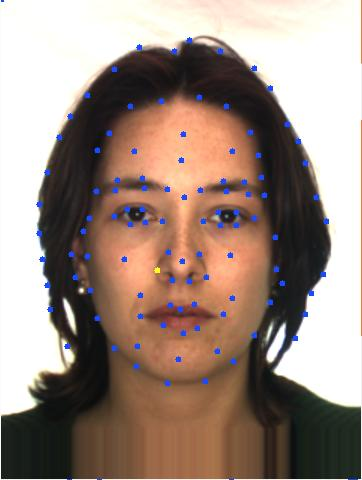
\includegraphics[width=0.25\linewidth]{Resources/manualmorph01.jpg}}
	\label{subfig:manualmorph01}\hspace{10pt}
	\subfloat[Morph no. 5]{%
		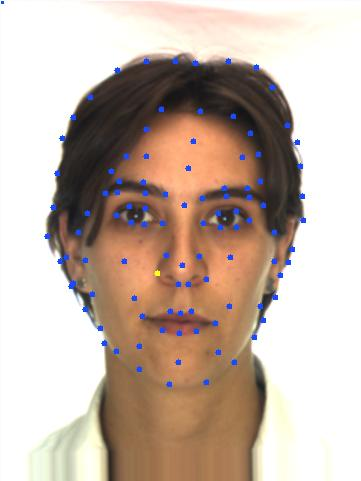
\includegraphics[width=0.25\linewidth]{Resources/manualmorph02.jpg}}
	\label{subfig:manualmorph02}\\
	\caption{Example of two ICAO compliant photos (1a and 1e) and morphs at stage 5 (1b), 15 (1c) and 25 (1d)}
	\label{fig:manual_morph} 
\end{figure}
In contrast to the automatic face morphing approach, manual morphing is discussed in this section. 

To achieve morphes, the open source software GNU Image Manipulation Software (GIMP) (Version 2.8.16) with the GIMP Animation Package (GAP) (Version 2.6) was selected for this process. Morphing with GAP follows the simple approach of manually placing connected landmarks at characterizing points in both faces. In \ref{fig:manual_morph} two pictures with a setup of landmarks are shown. It can be observed, that the landmarks are placed at characterizing points in both faces, e.g. at the eye browns, lips and nose. The general shape of the face as well as the shape of the head including the hair is also respected. In the example the facial landmarks are close to each other whereas the landmarks describing the shape of the hair are farer apart. 

The selection of characterizing points \todo{regions?} is based on findings \todo{erkenntnissen?} from earlier works on the topic of automatic face recognition, to achieve an optimal morphing result compared with own estimation based on the individual appearance of the subjects. \cite[60ff]{jain2008handbook} \cite{amos2016openface} \todo{DONE cite handbook of bio p.60} \todo{cite these fancy mp4 thingy}.
The algorithm shifts the landmarks from face one to face two. In addition to this the color of the skin is transmitted. 

%\subsubsection*{Morphing setup}
For the test samples 100 - 125 landmarks were placed, depending on the face characteristics. The output contains a sequence of 30 photos which show different stages of the morphing procedure. \ref{1e}


\subsubsection{Results}
\todo{compare to automatic results when there.}
\begin{figure}[h]
	\centering
	\subfloat[Subject 1]{%
		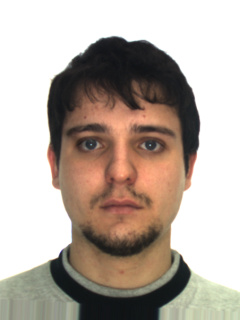
\includegraphics[width=0.19\linewidth]{Resources/p1.jpg}
	\label{1a}}\hfill
	\subfloat[Morph no. 5]{%
		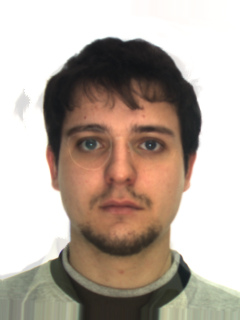
\includegraphics[width=0.19\linewidth]{Resources/m1.jpg}
	\label{1b}}\hfill
	\subfloat[Morph no. 15]{%
		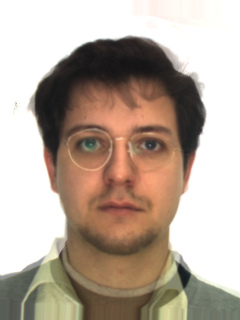
\includegraphics[width=0.19\linewidth]{Resources/m2.jpg}
	\label{foo}} \hfill
	\subfloat[Morph no. 25]{%
		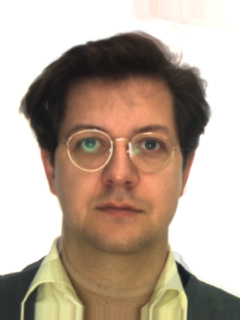
\includegraphics[width=0.19\linewidth]{Resources/m3.jpg}
	\label{1d}}\hfill
	\subfloat[Subject 2]{%
		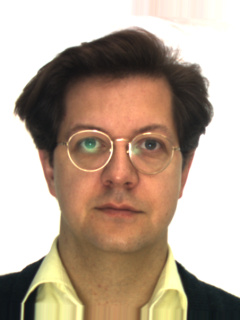
\includegraphics[width=0.19\linewidth]{Resources/p2.jpg}
	\label{1e} }
	\caption{Example of two ICAO compliant photos (\ref{1a} and \ref{1e}) and morphs at stage 5 (\ref{1b}), 15 (\ref{foo}) and 25 (\ref{1d})}
	\label{fig1} 
\end{figure}

In figure \ref{fig1} a two subjects and three morphing stages (5, 15 and 25) are shown. The visual inspection of \ref{1a} shows biometric features of both subjects whereas \subref{1e} and \ref{1d} has more similarity to the closer subject but also covers features of the other subject.
A manual post production of the morphs is not necessary because potential revealing details, like the interference \todo{?} of the clothes, glasses or hair is not considered by the algorithm.

\todo[inline]{OK Detailed description of the morphs}
\section{Face detection}

\subsection*{Detection algorithm} % alternativ Test setup?
As face detection algorithm the open source software OpenFace was selected. OpenFace is based on a neural network with is fully trained and has high confidence rates in the shipped version. Because OpenFaces main goal is to detect faces on arbitrary photos, the accuracy level is expected to be higher if it works on ICAO compliant data sets. 

\todo{ICAO compliance}

\subsection*{Process of work}
Both of the two source photos and the sequence of 30 morphs is given as input to the OpenFace comparison algorithm. OpenFace computes the match rate of every morph to both of the two photos. 
The expected outcome of comparison algorithm is an almost equal match rate for morph no. 15, where both pictures are represented to $50\%$. The closer the morph gets to one of the original pictures the higher the match rate and the lower to the other picture. 
\todo{mention match rates of sample pictures in fig 1}

\todo[inline]{hier distances abstrakt beschreiben}
\todo[inline]{beschreiben welcher thershold gewählt wurd und warum}

% !TeX root = main.tex
\section{Results}
Resulting from the work are the squared l2 euclidean distances calculated with the program OpenFace. The distance shows the similiarity to the given biometric references, it is a dissimilarity score. A lower distance means the compared two biometric references are more equal, when the distance is under a given threshold, these two biometric references are accepted to be the same biometric reference and so access is given. The resulting morphed photos were compared to diffrent photos of both biometric references, to get a independend distance. Which percentage of each biometric reference and the picture number is shown in \ref{percentageMorph}.
\subsection{Distances}

\subsubsection{Subset of 5 automatic generated morph sets (from biometric references also used by Budrhani)}\label{sec:subset5}
All resultingsquared l2 euclidean distances for the morphed photos of biometric references 01-m-002-27 to 01-m-003-24, 01-m-003-24 to 01-m-005-23, 01-m-004-23 to 01-m-005-23, 01-m-010-23 to 01-m-013-23 and 01-m-014-23 to 01-m-016-23 compared to the corresponding compare images are way too much data. So there is as an example of the morphed image 01-m-002-27 - 01-m-003-24:

\begin{tabular}{lrrrrrr}
	Picture & 01-m-002-28 & 01-m-002-29 & 01-m-002-30 & 01-m-003-25 & 01-m-003-26 & 01-m-003-27 \\
	 & & & & & & \\
	1 & 0.11916 & 0.07499 & 0.19188 & 1.30874 & 1.16709 & 1.31322\\
	2 & 0.13701 & 0.06885 & 0.18756 & 1.25716 & 1.10248 & 1.25841\\ 
	3 & 0.17384 & 0.06523 & 0.19060 & 1.17656 & 1.01354 & 1.17311\\ 
	4 & 0.22901 & 0.07982 & 0.21253 & 1.08009 & 0.90457 & 1.06856\\ 
	5 & 0.31766 & 0.12439 & 0.24763 & 0.89989 & 0.70834 & 0.88006\\ 
	6 & 0.39700 & 0.16766 & 0.30990 & 0.83492 & 0.62518 & 0.81035\\ 
	7 & 0.50975 & 0.24823 & 0.40167 & 0.72848 & 0.51501 & 0.70676\\ 
	8 & 0.67400 & 0.39087 & 0.53792 & 0.60985 & 0.39251 & 0.59632\\ 
	9 & 0.74737 & 0.46525 & 0.58010 & 0.52552 & 0.32146 & 0.50314\\ 
	10 & 0.94108 & 0.62628 & 0.74969 & 0.40924 & 0.21060 & 0.37129\\ 
	11 & 1.05918 & 0.76321 & 0.86483 & 0.32472 & 0.13804 & 0.28219\\ 
	12 & 1.21209 & 0.90143 & 0.99503 & 0.25177 & 0.08833 & 0.20977\\ 
	13 & 1.25246 & 0.97993 & 1.05583 & 0.19876 & 0.05832 & 0.17236\\ 
	14 & 1.34758 & 1.07654 & 1.14637 & 0.19252 & 0.04679 & 0.16232\\ 
	15 & 1.37122 & 1.13813 & 1.18339 & 0.14941 & 0.05522 & 0.13605\\ 
\end{tabular}\\

Also shown in figure \ref{fig:Result1}.

The results of the 01-m-002-27 to 01-m-003-24, 01-m-003-24 to 01-m-005-23, 01-m-004-23 to 01-m-005-23, 01-m-010-23 to 01-m-013-23 and 01-m-014-23 to 01-m-016-23 morphs are shown in figure \ref{fig:Result1-5}.

For better recognizability the mean value of all the diffrent squared l2 euclidean distances is calculated for biometric reference 1 and biometric reference 2. The result is shwon in figure \ref{fig:Result1-5-mean}. The distance graphs crosses by ($9.04$, $0.49$), so the best distance for both biometric references is with picture 9 with distances of $0.48$ and $0.49$. Picture 9 with $42.86$\% of biometric reference 1 and $57.14$\% of biometric reference 2 so it  not the middle of all 15 pictures, this could be the cause of the different distances of the biometric references to their own compare images.

OpenFace uses normally a threshold of \textbf{$0.99$}, which allows nearly all morphs from picture 5 to 10 to be successful acknowledged as shown in figure \ref{fig:Result1-5}. Only in 3 cases there is the distance way too high to work properly. The compare pictures are 01-m-016-24.jpg, 01-m-016-25.jpg and 01-m-016-26.jpg which are all from the same biometric reference, so this morph with this biometric reference is not working, this could be the cause of the different distances to the own compare images. As a result in 4 out of 5 cases it is possible to morph two biometric references to be successful acknowledged, this makes a success chance of $80$\%.

\begin{figure}[htbp] 
	\centering
		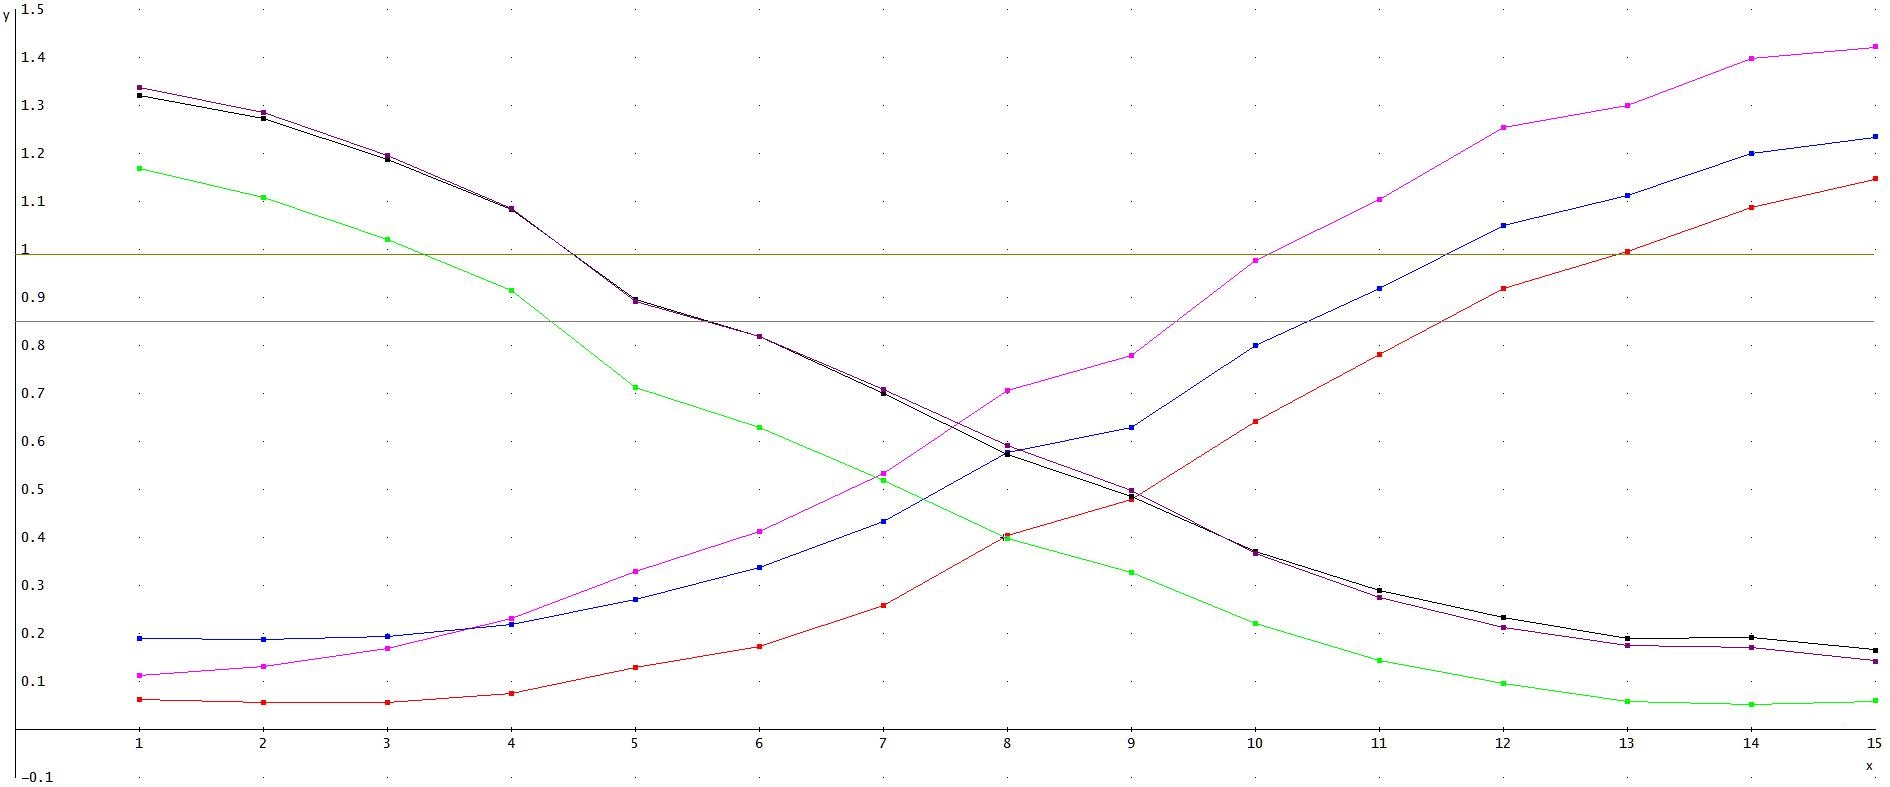
\includegraphics[width=0.95\textwidth]{Resources/result1.jpg}
	\caption{Squared l2 euclidean distances (y axis) of morphs from 01-m-002-27 to 01-m-003-24 (with 15 steps ont he x axis) comparing to 01-m-002-28.jpg, 01-m-002-29.jpg, 01-m-002-30.jpg, 01-m-003-25.jpg, 01-m-003-26.jpg and 01-m-003-27.jpg}
	\label{fig:Result1}
\end{figure}

\begin{figure}[htbp] 
	\centering
		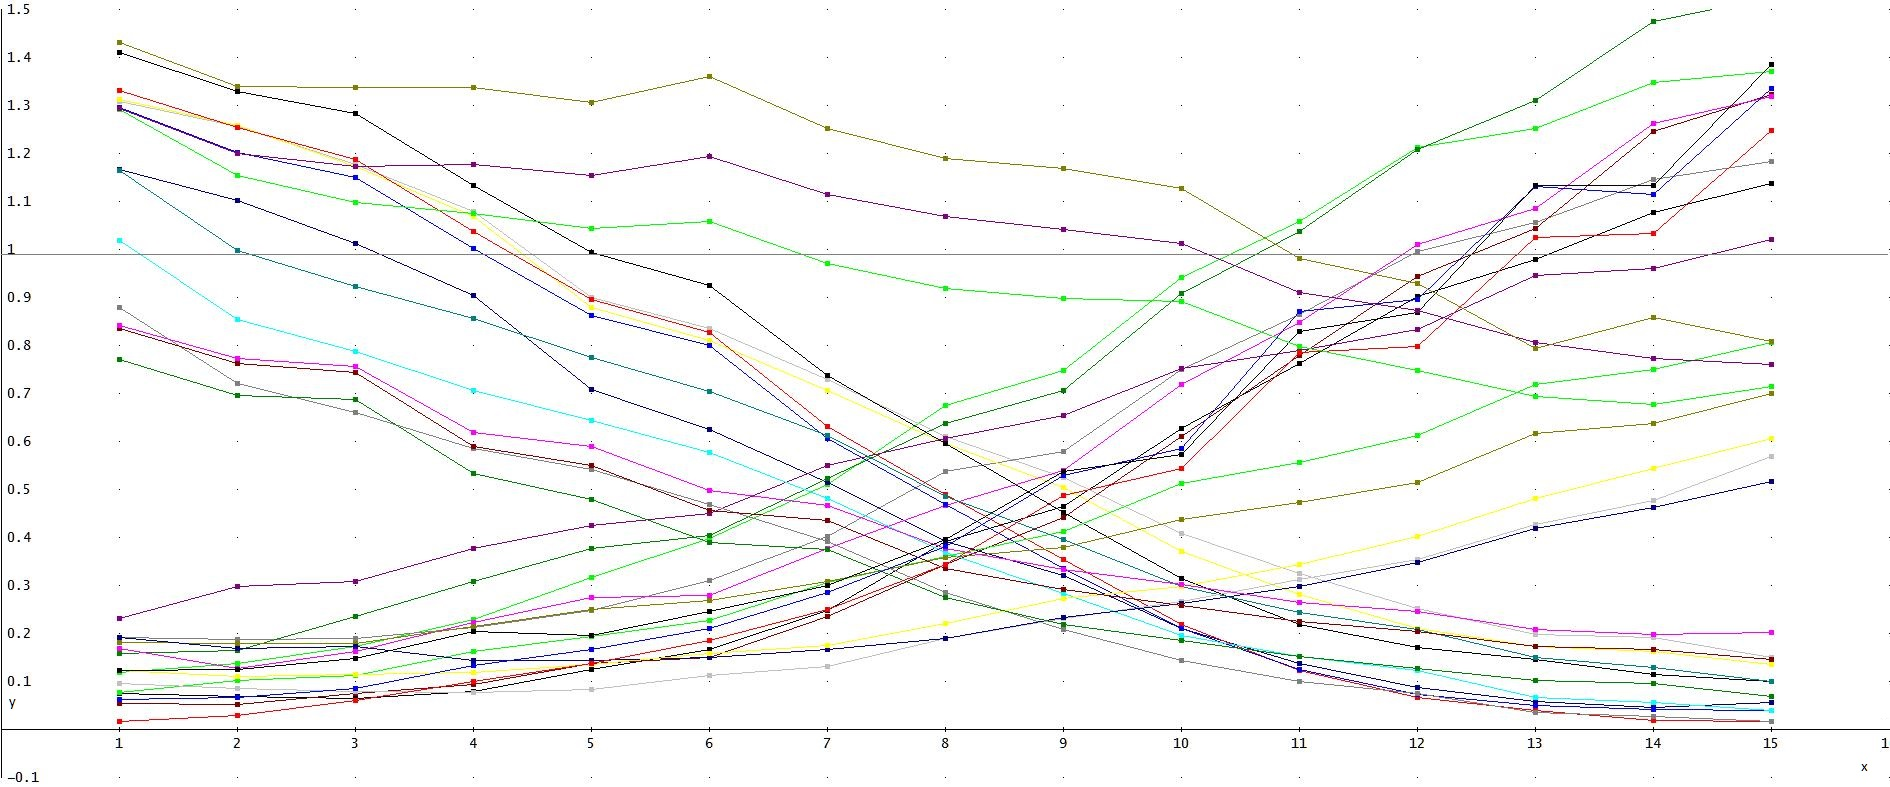
\includegraphics[width=0.95\textwidth]{Resources/result1-5.jpg}
	\caption{Squared l2 euclidean distances (y axis) of morphs from 01-m-002-27 to 01-m-003-24, 01-m-003-24 to 01-m-005-23, 01-m-004-23 to 01-m-005-23, 01-m-010-23 to 01-m-013-23 and 01-m-014-23 to 01-m-016-23 (with 15 steps on the x axis) comparing to the corresponding compare photos}
	\label{fig:Result1-5}
\end{figure}

\begin{figure}[htbp] 
	\centering
		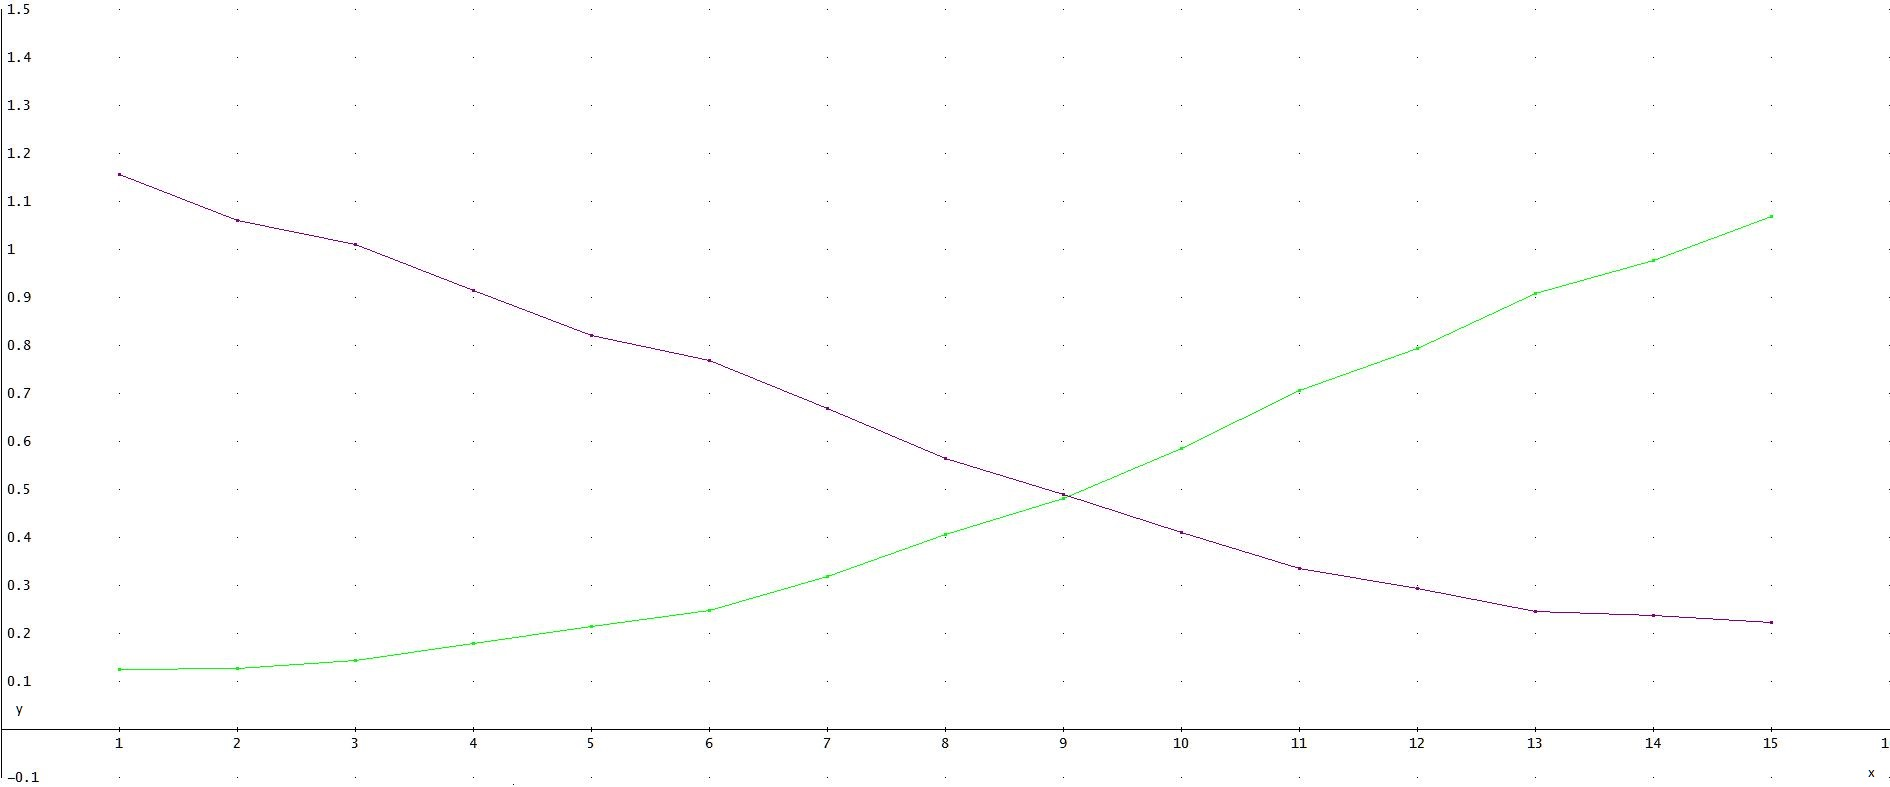
\includegraphics[width=0.95\textwidth]{Resources/result1-5-mean.jpg}
	\caption{Mean squared l2 euclidean distances (y axis) of morphs from 01-m-002-27 to 01-m-003-24, 01-m-003-24 to 01-m-005-23, 01-m-004-23 to 01-m-005-23, 01-m-010-23 to 01-m-013-23 and 01-m-014-23 to 01-m-016-23 (with 15 steps on the x axis) comparing to the corresponding compare photos}
	\label{fig:Result1-5-mean}
\end{figure}
\newpage
\subsubsection{Subset of 39 automatic generated morph sets}\label{sec:subset39}
Now 39 automatic generated sets of morphed biometric references were used. The used biometric references are:
\begin{multicols}{3}
\begin{itemize}
\item 01-m-002 - 01-m-003
\item 01-m-003 - 01-m-004
\item 01-m-004 - 01-m-005
\item 01-m-013 - 01-m-014
\item 01-m-016 - 01-m-017
\item 01-m-019 - 01-m-020
\item 01-m-020 - 01-m-021
\item 01-m-021 - 01-m-022
\item 01-m-022 - 01-m-023
\item 01-m-025 - 01-m-026
\item 01-m-026 - 01-m-027
\item 01-m-030 - 01-m-031
\item 01-m-031 - 01-m-032
\item 01-m-032 - 01-m-033
\item 01-m-037 - 01-m-038
\item 01-m-038 - 01-m-039
\item 01-m-039 - 01-m-040
\item 01-m-040 - 01-m-041
\item 01-m-041 - 01-m-042
\item 01-m-042 - 01-m-043
\item 01-m-043 - 01-m-044
\item 01-m-044 - 01-m-045
\item 01-m-045 - 01-m-046
\item 01-m-046 - 01-m-047
\item 01-m-047 - 01-m-048
\item 01-m-048 - 01-m-049
\item 01-m-051 - 01-m-052
\item 01-m-052 - 01-m-053
\item 01-m-053 - 01-m-054
\item 01-m-054 - 01-m-055
\item 01-m-055 - 01-m-056
\item 01-m-059 - 01-m-060
\item 01-m-060 - 01-m-061
\item 01-m-065 - 01-m-066
\item 01-m-066 - 01-m-067
\item 01-m-069 - 01-m-070
\item 01-m-072 - 01-m-073
\item 01-m-073 - 01-m-074
\item 01-m-074 - 01-m-075
\end{itemize}
\end{multicols}


With these sets again the squared l2 euclidean distances are computed to the associated compare images of the two biometric references. The resulting distances are shown in figure \ref{fig:Result39-all}. To decrease the amount of information the mean values for both biometric references were computed and are shown in figure \ref{fig:Result39-mean}. The distance graphs crosses by ($7.93$, $0.6$), so the best distance for both biometric references is with picture 8 with distances of $0.6$ and $0.59$. Picture 8 is the exact middle of all 15 pictures with $50$\% of biometric reference 1 and $50$\% of biometric reference 2.
\begin{figure}[htbp] 
	\centering
		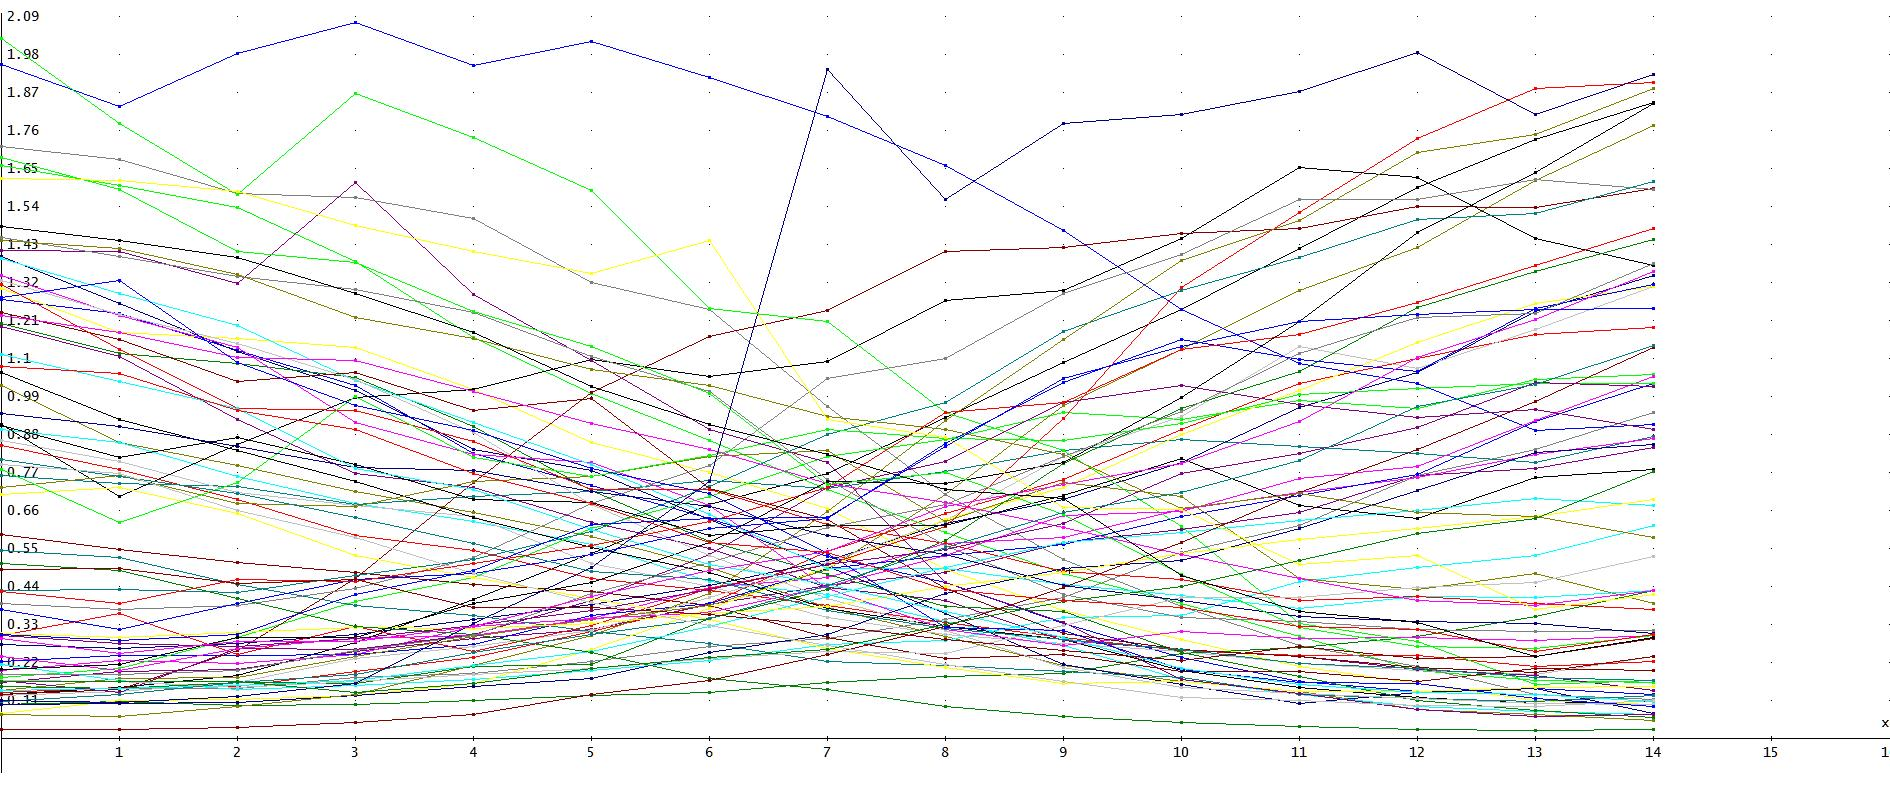
\includegraphics[width=0.95\textwidth]{Resources/result39-all.jpg}
	\caption{Squared l2 euclidean distances (y axis) of the subset of 39 morphs (with 15 steps on the x axis) comparing to the corresponding compare photos}
	\label{fig:Result39-all}
\end{figure}
\begin{figure}[htbp] 
	\centering
		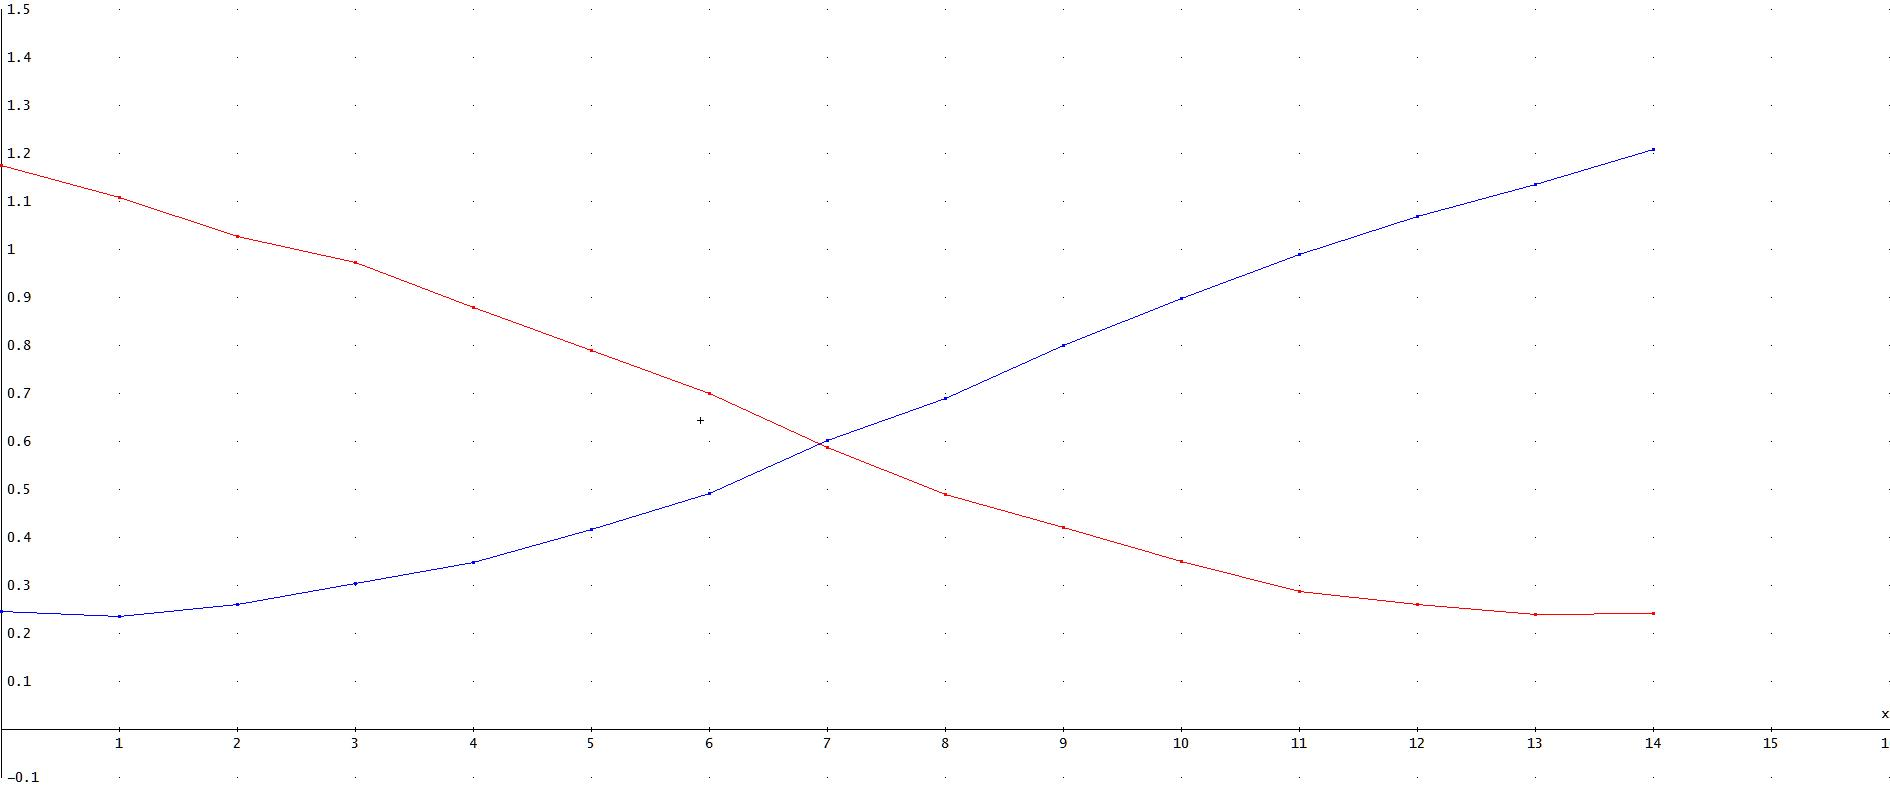
\includegraphics[width=0.95\textwidth]{Resources/result39-mean.jpg}
	\caption{Mean squared l2 euclidean distances (y axis) of the subset of 39 morphs (with 15 steps on the x axis) comparing to the corresponding compare photos}
	\label{fig:Result39-mean}
\end{figure}

\newpage
\subsubsection{Subset of 8 manual generated morph sets}
\label{sec:subsetman}
Finally 8 sets of morphed biometric references were created and the distances to the comparing images was calculated. As a speciality in this set a morph of a woman and a man.
The biometric references for the manual morphing are:
\begin{multicols}{2}
\begin{itemize}
\item 01-m-002-27 - 01-m-003-24
\item 01-m-003-24 - 01-m-005-23
\item 01-m-004-23 - 01-m-005-23
\item 01-m-010-23 - 01-m-013-23
\item 01-m-014-23 - 01-m-016-23
\item 01-m-017-23 - 01-m-019-23
\item 01-m-020-23 - 01-w-002-23
\item 01-w-036-23 - 01-w-037-23
\end{itemize}
\end{multicols}
For this subset the squared l2 euclidean distances to the associated compare images of the two biometric references is also computed. The resulting distances are shown in figure \ref{fig:result-jannis-all}. To decrease the amount of information the mean values for both biometric references were computed and are shown in figure \ref{fig:result-jannis-mean}.

\begin{figure}[htbp] 
	\centering
		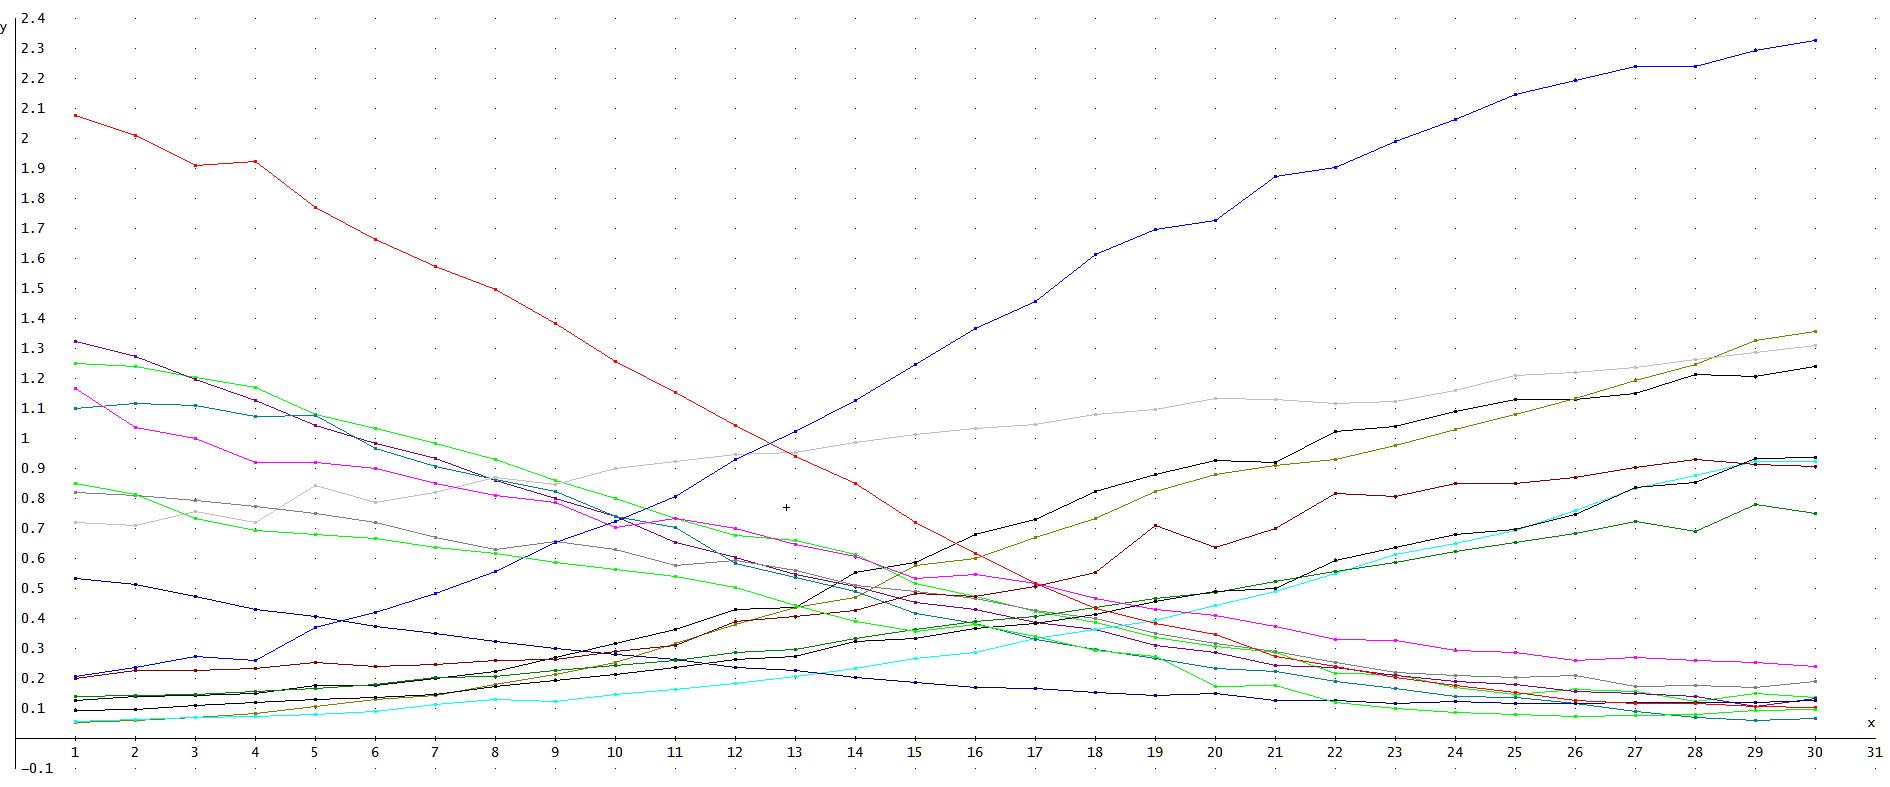
\includegraphics[width=0.95\textwidth]{Resources/result-jannis.jpg}
	\caption{Squared l2 euclidean distances (y axis) comparing to the corresponding compare photos of the subset of 8 manual morphs (with 30 steps on the x axis)}
	\label{fig:result-jannis-all}
\end{figure}
\begin{figure}[htbp] 
	\centering
		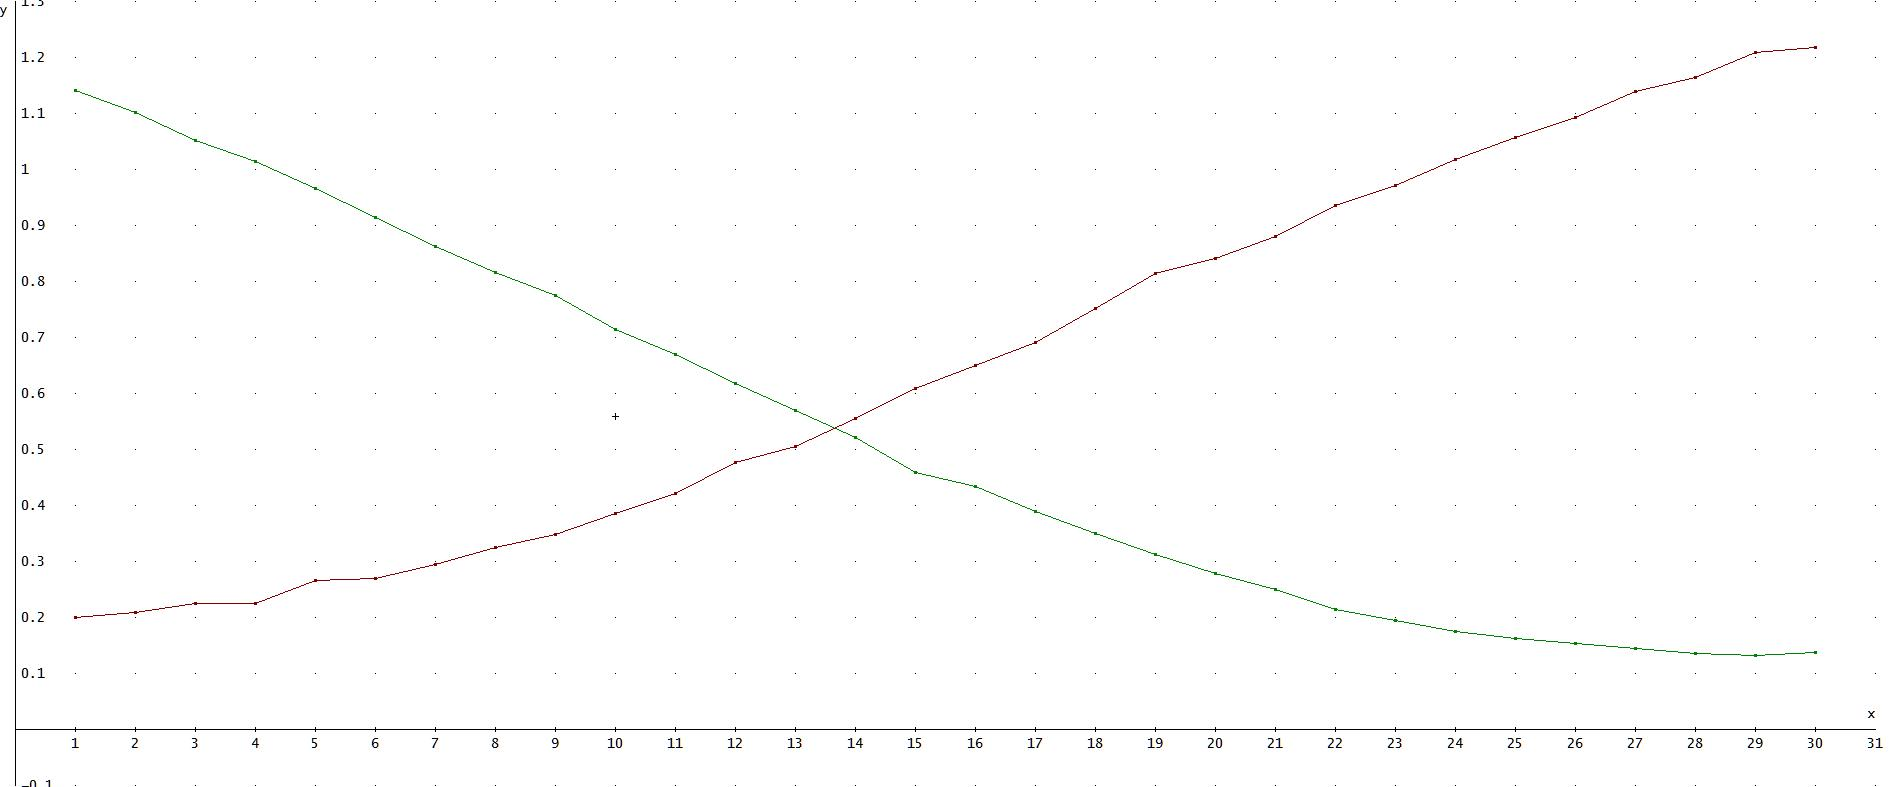
\includegraphics[width=0.95\textwidth]{Resources/result-jannis-mean}
	\caption{Mean squared l2 euclidean distances (y axis) comparing to the corresponding compare photos of the subset of 8 manual morphs (with 30 steps on the x axis)}
	\label{fig:result-jannis-mean}
\end{figure}

\newpage
\subsection{Threshold}
As a result a threshold is computed to get a $10$\% biometric false acceptance of an impostor (false match rate (FMR)) and a $90$\% chance to non-match a morphed image.

\subsubsection{Automatic morphing (Subset of 39 automatic generated morph sets)}\label{sec:automorph-thres}
For the calculation of the threshold of the automatic generated morphs the subset of 39 of section \ref{sec:subset39} is used, it's bigger than the subset of 5 automatic generated morph sets (from biometric references also used by Budrhani) of section \ref{sec:subset5} so the used mean values are more representative.
Used for the calculation are the squared l2 euclidean distances of section \ref{sec:subset39}.
The resulting threshold for this subset is \textbf{$0.76891524$}. In contrast to the distances it is shown in figure \ref{fig:Result39-90-10}.


\begin{figure}[htbp] 
	\centering
		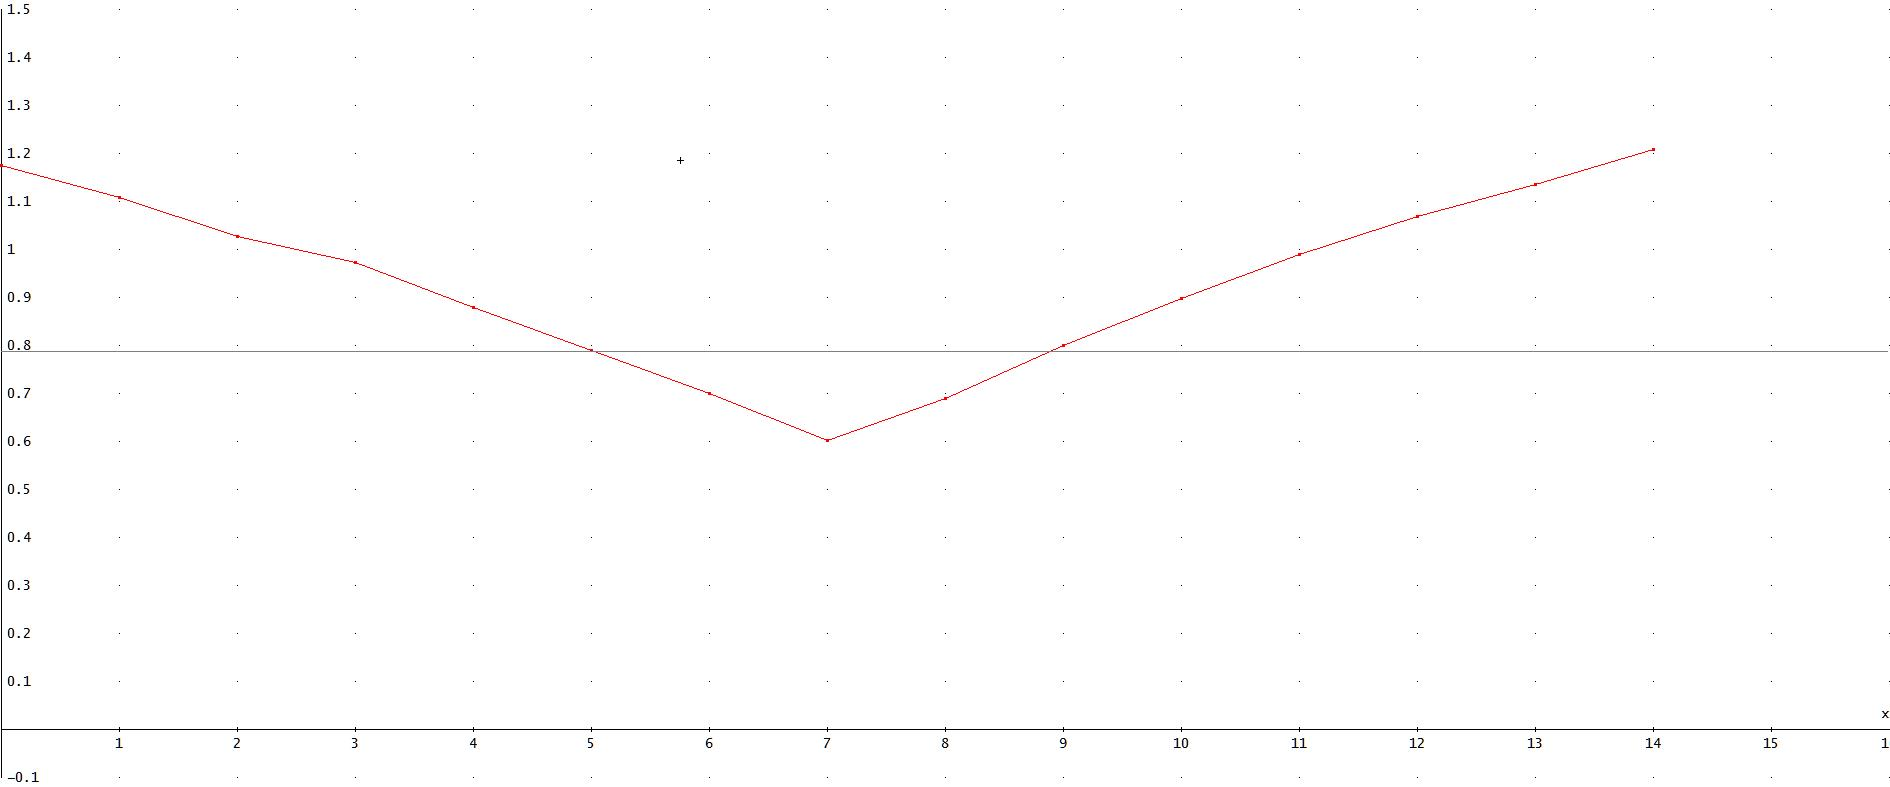
\includegraphics[width=0.95\textwidth]{Resources/result39-90-10.jpg}
	\caption{Squared l2 euclidean distances (y axis) of the 39 morphed subset (with 15 steps on the x axis) compared to the corresponding compare photos, in contrast to the calculated threshold of $0.76891524$} %\todo{beschreibung anpassen}
	\label{fig:Result39-90-10}
\end{figure}

\subsubsection{Manual morphing (Subset of 8 manual generated morph sets)}\label{sec:manmorph-thres}
For the calculation of the threshold of the manual generated morphs the subset of 8 of section \ref{sec:subsetman} is used and the calculated distances from the same section.
The resulting threshold for this subset is \textbf{$0.7172467154$}. In contrast to the distances it is shown in figure \ref{fig:Resultman-90-10}.


\begin{figure}[htbp] 
	\centering
		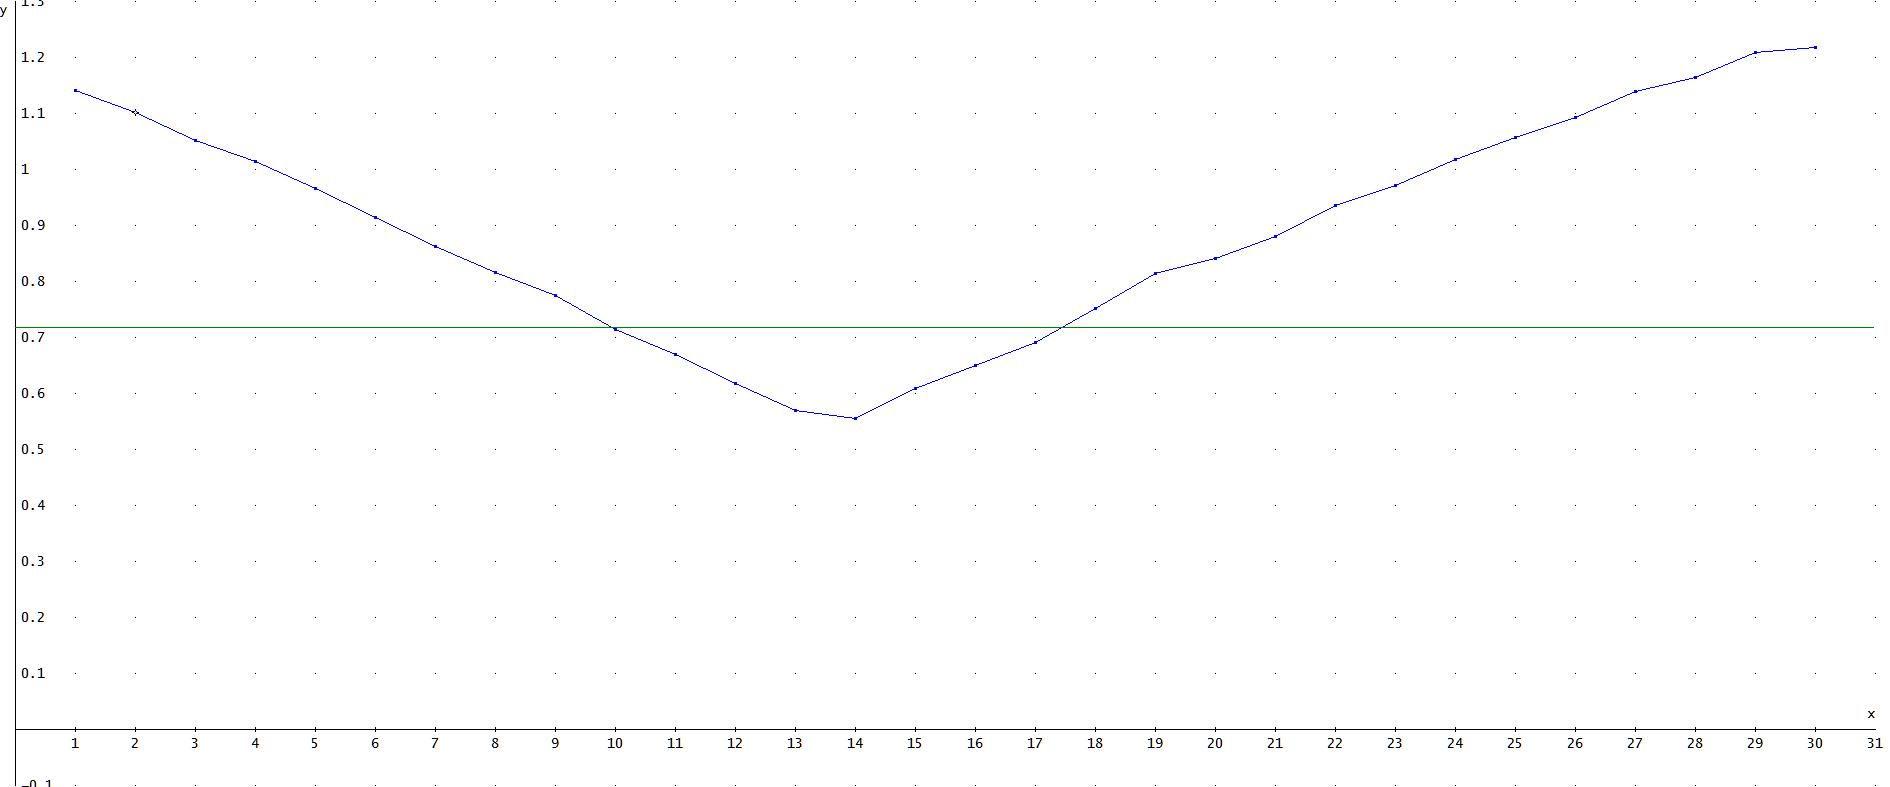
\includegraphics[width=0.95\textwidth]{Resources/result-jannis-mean-90-10.jpg}
	\caption{Squared l2 euclidean distances (y axis) of the 8 manual morphed subset (with 30 steps on the x axis) compared to the corresponding compare photos, in contrast to the calculated threshold of $0.7172467154$} %\todo{beschreibung anpassen}
	\label{fig:Resultman-90-10}
\end{figure}

\subsubsection{Comparison threshold of manual and automatic}\label{sec:comp-thres}
The two tresholds of the automatic morphing from \ref{sec:automorph-thres} $0.76891524$ and the manual morphing \ref{sec:manmorph-thres} $0.7172467154$ are close to another. They differ only about $0.05$, which is not much. The threshold of the manual morphing is lower than the automatic threshold, this could mean that the images of the manual morphing are better, but such a low difference could also be possible through lower the distances because of the input biometric reference variations.

As a result the threshold of OpernFace should be set to $0.71$ to fight off morphing attacks, in case the biometric false rejection rate in the biometric system is acceptable.
\section{Conclusion}

It takes about 40 minutes to achieve a high quality manual morph with GIMP GAP. 
\section{Further topics}
\todo[inline]{ungemorpht vorvergleichen}
\todo[inline]{Morphen von mehreren bildern}
\todo[inline]{Visual inspection}

% needed in second column of first page if using \IEEEpubid
%\IEEEpubidadjcol

% An example of a floating figure using the graphicx package.
% Note that \label must occur AFTER (or within) \caption.
% For figures, \caption should occur after the \includegraphics.
% Note that IEEEtran v1.7 and later has special internal code that
% is designed to preserve the operation of \label within \caption
% even when the captionsoff option is in effect. However, because
% of issues like this, it may be the safest practice to put all your
% \label just after \caption rather than within \caption{}.
%
% Reminder: the "draftcls" or "draftclsnofoot", not "draft", class
% option should be used if it is desired that the figures are to be
% displayed while in draft mode.
%
%\begin{figure}[!t]
%\centering
%\includegraphics[width=2.5in]{myfigure}
% where an .eps filename suffix will be assumed under latex, 
% and a .pdf suffix will be assumed for pdflatex; or what has been declared
% via \DeclareGraphicsExtensions.
%\caption{Simulation Results}
%\label{fig_sim}
%\end{figure}

% Note that IEEE typically puts floats only at the top, even when this
% results in a large percentage of a column being occupied by floats.


% An example of a double column floating figure using two subfigures.
% (The subfig.sty package must be loaded for this to work.)
% The subfigure \label commands are set within each subfloat command, the
% \label for the overall figure must come after \caption.
% \hfil must be used as a separator to get equal spacing.
% The subfigure.sty package works much the same way, except \subfigure is
% used instead of \subfloat.
%
%\begin{figure*}[!t]
%\centerline{\subfloat[Case I]\includegraphics[width=2.5in]{subfigcase1}%
%\label{fig_first_case}}
%\hfil
%\subfloat[Case II]{\includegraphics[width=2.5in]{subfigcase2}%
%\label{fig_second_case}}}
%\caption{Simulation results}
%\label{fig_sim}
%\end{figure*}
%
% Note that often IEEE papers with subfigures do not employ subfigure
% captions (using the optional argument to \subfloat), but instead will
% reference/describe all of them (a), (b), etc., within the main caption.


% An example of a floating table. Note that, for IEEE style tables, the 
% \caption command should come BEFORE the table. Table text will default to
% \footnotesize as IEEE normally uses this smaller font for tables.
% The \label must come after \caption as always.
%
%\begin{table}[!t]
%% increase table row spacing, adjust to taste
%\renewcommand{\arraystretch}{1.3}
% if using array.sty, it might be a good idea to tweak the value of
% \extrarowheight as needed to properly center the text within the cells
%\caption{An Example of a Table}
%\label{table_example}
%\centering
%% Some packages, such as MDW tools, offer better commands for making tables
%% than the plain LaTeX2e tabular which is used here.
%\begin{tabular}{|c||c|}
%\hline
%One & Two\\
%\hline
%Three & Four\\
%\hline
%\end{tabular}
%\end{table}


% Note that IEEE does not put floats in the very first column - or typically
% anywhere on the first page for that matter. Also, in-text middle ("here")
% positioning is not used. Most IEEE journals use top floats exclusively.
% Note that, LaTeX2e, unlike IEEE journals, places footnotes above bottom
% floats. This can be corrected via the \fnbelowfloat command of the
% stfloats package.



%\section{Conclusion}
%\blindtext





% if have a single appendix:
%\appendix[Proof of the Zonklar Equations]
% or
%\appendix  % for no appendix heading
% do not use \section anymore after \appendix, only \section*
% is possibly needed

% use appendices with more than one appendix
% then use \section to start each appendix
% you must declare a \section before using any
% \subsection or using \label (\appendices by itself
% starts a section numbered zero.)
%


%\appendices
%\section{Proof of the First Zonklar Equation}
%\blindtext

% use section* for acknowledgement
%\section*{Acknowledgment}


%The authors would like to thank...


% Can use something like this to put references on a page
% by themselves when using endfloat and the captionsoff option.
\ifCLASSOPTIONcaptionsoff
  \newpage
\fi



% trigger a \newpage just before the given reference
% number - used to balance the columns on the last page
% adjust value as needed - may need to be readjusted if
% the document is modified later
%\IEEEtriggeratref{8}
% The "triggered" command can be changed if desired:
%\IEEEtriggercmd{\enlargethispage{-5in}}

% references section

% can use a bibliography generated by BibTeX as a .bbl file
% BibTeX documentation can be easily obtained at:
% http://www.ctan.org/tex-archive/biblio/bibtex/contrib/doc/
% The IEEEtran BibTeX style support page is at:
% http://www.michaelshell.org/tex/ieeetran/bibtex/
%\bibliographystyle{IEEEtran}
% argument is your BibTeX string definitions and bibliography database(s)
%\bibliography{IEEEabrv,../bib/paper}
%
% <OR> manually copy in the resultant .bbl file
% set second argument of \begin to the number of references
% (used to reserve space for the reference number labels box)
%\begin{thebibliography}{1}

%\bibitem{IEEEhowto:kopka}
%H.~Kopka and P.~W. Daly, \emph{A Guide to \LaTeX}, 3rd~ed.\hskip 1em plus
%  0.5em minus 0.4em\relax Harlow, England: Addison-Wesley, 1999.

%\end{thebibliography}
\bibliography{Quellen} 

% biography section
% 
% If you have an EPS/PDF photo (graphicx package needed) extra braces are
% needed around the contents of the optional argument to biography to prevent
% the LaTeX parser from getting confused when it sees the complicated
% \includegraphics command within an optional argument. (You could create
% your own custom macro containing the \includegraphics command to make things
% simpler here.)
%\begin{biography}[{\includegraphics[width=1in,height=1.25in,clip,keepaspectratio]{mshell}}]{Michael Shell}
% or if you just want to reserve a space for a photo:

\begin{IEEEbiography}[{\includegraphics[width=1in,height=1.25in,clip,keepaspectratio]{picture}}]{John Doe}
\blindtext
\end{IEEEbiography}

% You can push biographies down or up by placing
% a \vfill before or after them. The appropriate
% use of \vfill depends on what kind of text is
% on the last page and whether or not the columns
% are being equalized.

%\vfill

% Can be used to pull up biographies so that the bottom of the last one
% is flush with the other column.
%\enlargethispage{-5in}




% that's all folks
\end{document}


